\section{Algorithm verification}
\todo[inline]{initial test of A and X on toy example}
In this section the implementation of Cov-DL and M-SBL are verified separately based on the MSE between the true and the estimated matrices.

\subsection{Test of Cov-DL}
To test 	



With the implemented algorithms, Cov-DL and M-SBL, the purpose is now to investigate the performance of each algorithm. The performance will be measure by a error measure -- the mean square error (MSE) -- this will be presented in the next section. 
All the tests will be done one the estimated matrices but for the comparison of these error measurements the true mixing matrix will be used. 
As the true $\mathbf{A}$ is used we can not compared the performance of Cov-DL but only M-SBL. 
The Cov-DL algorithm will instead be tested for different choice of parameters, the initial $\mathbf{A}_{\text{ini}}$ using in the Cov-DL for the optimisation part of finding the matrix $\mathbf{D}$, and the number of segment in Cov-DL.

The goal with all these tests is make the best choice for each parameters, to achieve lowest error, such that when the baseline algorithm is used on realistic data set, the EEG measurements, the parameters as been chosen with the best performance in mind -- leading to the best scenario of finding the true mixing matrix and source matrix from EEG measurements.

First of all, we will run a test, with random setting, to see how the error margin is for both algorithms.
\todo[inline]{Dette afsnit virker som om det skal komme efter vi har beskrevet implementeringen af koden/flowdiagrammet.\\
Vi skriver at vi ikke kan compare performnce på Cov-DL, det passer vel ikke den bliver sammen lignet med den rigtige $\textbf{A}$ og hertil skruer vi så på $\textbf{A}_{init}$ og cos-seg for at se hvordan det påvirker resultatet.\\
måler vi en error margin som nævnt tilsidst?}


\subsection{Tests}

Before any testing of the performance of the algorithms we will test if the algorithms give us a reasonable result\todo{hvad er forskellen her?}. The Cov-DL and M-SBL has been tested with the simple data to see if the algorithms give us a results and how the performance of M-SBL differs when using an estimated mixing matrix and the true mixing matrix\todo{syntes vi skal holde de to adskildt endnu. der er ikke nogen grund til at anvende $\textbf{A}_{rec}$ inden vi har kigget på dens fejl. ville det give mening at plotte $\textbf{A}$?}.

In the following figure we see the recovered sources aligned with the real source of a system with $M = 3$ and $k = 4$ for $L = 100$ -- a small system.
\begin{figure}[H]
    \begin{minipage}{0.5\linewidth}
    	\centering
        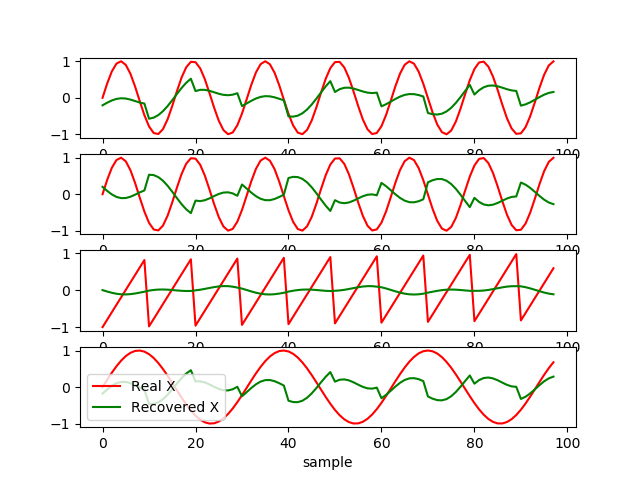
\includegraphics[scale=0.5]{figures/chapter6/test_of_algo_mix_data.png}
		\subcaption{}
    \end{minipage} 
    ~\hfill~
    \begin{minipage}{0.5\linewidth}
    	\centering
        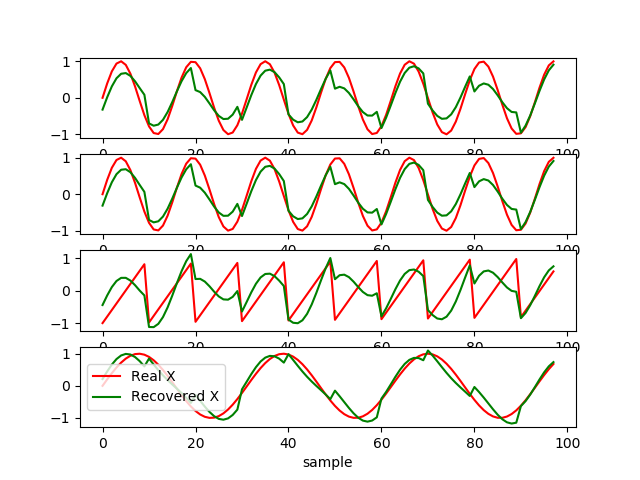
\includegraphics[scale=0.5]{figures/chapter6/test_of_algo_mix_data_realA.png}
        \subcaption{}
    \end{minipage}
    \caption{(a) The $k$ recovered sources from M-SBL with the estimated mixing matrix $\mathbf{A}$ and (b) the real mixing matrix $\mathbf{A}$}
    \label{fig:test_toy}
\end{figure}
\noindent
From figure \ref{fig:test_toy}.a we see that four signal (our sources) has been recovered which is identical with the number of sources in the simple data set. Furthermore, we see that the estimation of the sources are not identical with the real sources but follow some patterns of the real sources. For example source one and two in \ref{fig:test_toy}.a increase and decrease at the same samples but not with the same amplitude as the estimated sources are more constant like than the sinus signals which is the real sources. Source three look more like a sinus signal than a sawtooth signal. The last source do not look like the sinus signal.
In figure \ref{fig:test_toy}.b the real mixing matrix is used when estimating the source matrix with M-SBL. Here we see that sources look more like the real sources expect source three.
To compare the two estimation of the source matrix $\mathbf{X}$ the MSE has been applied:
\begin{table}[H]
\centering
\begin{tabular}{|c|c|c|}
\hline
         & Estimated $\mathbf{A}$ & Real $\mathbf{A}$ \\ \hline
MSE of $\mathbf{A}$ & 2.16 & $\times$ \\ 
\hline 
MSE of $\mathbf{X}$ & 0.49 & 0.14 \\ 
\hline
\end{tabular} 
\caption{MSE values of the mixing matrix $\mathbf{A}$ and source matrix $\mathbf{X}$ from the Simple Data Set}
\label{tab:test}
\end{table}
\noindent
From \ref{tab:test} we see that the estimated source matrix has low MSE value. This is due to the low value in $\mathbf{X}$ that the error also is small. But we see a different between the used of a estimated mixing matrix and the real mixing matrix.


\section{Test on AR data}
\todo[inline]{insert test of A plus variable adjustment, and test of X on AR data}
\section{Parameter Choice}
\begin{enumerate}
\item Describe why we want to set $N = k$, logical discussion. No results yet to back up the assuming.
	\begin{itemize}
	\item The amount of $N$ is unknown as it change for every brain
	\item Therefore, we do not know the amount of activation inside the brain, but it those there are of interest in this thesis.
	\end{itemize}
\item Talk about the parameter choice for $M$ and $N$ -- a low-density system have what? $M =  8$ and $N = 16$ or $N = 32$.
\end{enumerate}
 

\subsubsection{Initial A in Cov-DL}
For the Cov-DL algorithm when estimating the mixing matrix $\mathbf{A}$ a matrix $\mathbf{D}$ is used in the recovering process. For a over-determined system \ref{sec:over_det} $\mathbf{D}$ is found from an optimisation problem \eqref{eq:Cov_DL2} created with use of principal component analysis. To solve the optimization problem and finding $\mathbf{D}$ an initial $\mathbf{A}_{\text{ini}}$ is used as a starting point in the optimization process. The choice of this initial $\mathbf{A}_{\text{ini}}$ will affect how the good an estimate our recovered mixing matrix $\mathbf{A}$ is.

In this section we will be testing three different choice for $\mathbf{A}_{\text{ini}}$:
\begin{itemize}
\item[-] A matrix $\mathbf{A1}$ drawn from a continuous uniform distribution in the half-open interval $[0.0, 1.0)$
\item[-] A matrix $\mathbf{A2}$ drawn from a uniform distribution in the half-open interval $[-1.0, 1.0)$
\item[-] A matrix $\mathbf{A3}$ drawn from a Gaussian distribution with mean 0 and variance 1
\end{itemize}
The test of different initial $\mathbf{A}_{\text{ini}}$ will be performed on the both data sets presented in \ref{sec:dataset}. The goal with this test is to find the best initial $\mathbf{A}_{\text{ini}}$. The results are based on MSE of both the Cov-DL with $\mathbf{A}_{\text{ini}}$ and the M-SBL which used the recovered $\mathbf{A}$ as input and therefore also is affect by the choice of $\mathbf{A}_{\text{ini}}$.

When it comes to finding the best initial $\mathbf{A}_{\text{ini}}$ it must be taken into account that the realistic data set -- the EEG measurements -- are more random distributed and have higher amplitude than our simple data set so we are more likely to look at the result for the autoregressive data set as it more resembling the EEG measurements. This lead to that the choice for $\mathbf{A}_{\text{ini}}$ may have a higher error in the simple data set than the autoregressive data set.

For the test we are looking at a system of size $M = 8$, $k = 16$ and $L = 1000$. Furthermore, for the Cov-DL the data has been divided in segments of 10 samples leading to 100 segments.
\begin{figure}[H]
\centering
    \begin{minipage}[t]{.45\textwidth}
        \centering
		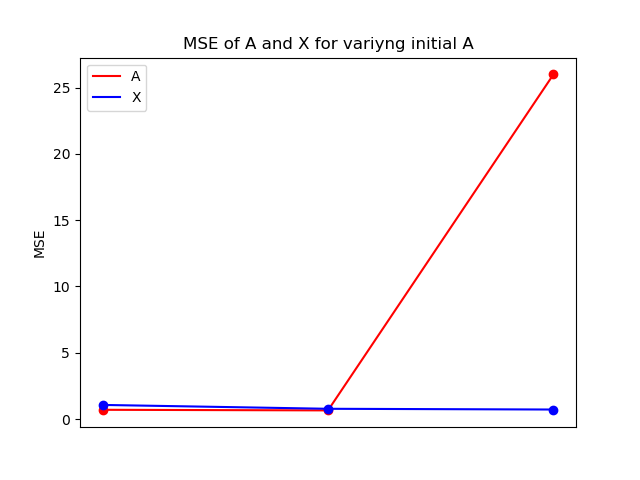
\includegraphics[scale=0.5]{figures/chapter6/Mix_Error_initial_A_m8_k16_L1000.png}
		\subcaption{Simple Data Set - Estimated A}
    \end{minipage} 
    \hfill
    \begin{minipage}[t]{.45\textwidth}
        \centering
		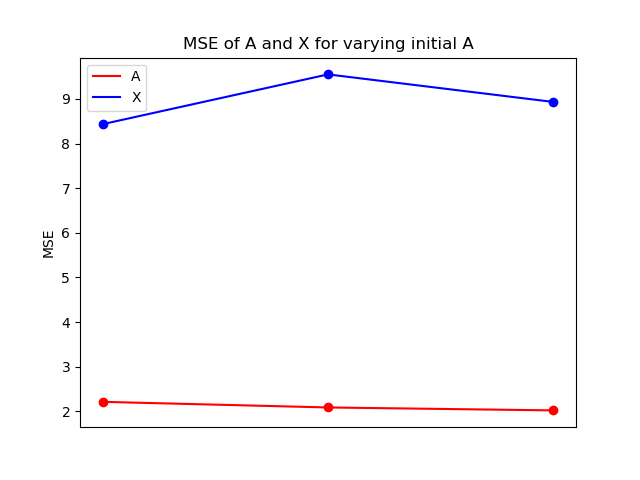
\includegraphics[scale=0.5]{figures/chapter6/AR_Error_initial_A_m8_k16_L1000.png}
		\subcaption{Autoregressive Data Set - Estimated A}
    \end{minipage}
    \begin{minipage}[t]{.45\textwidth}
        \centering
		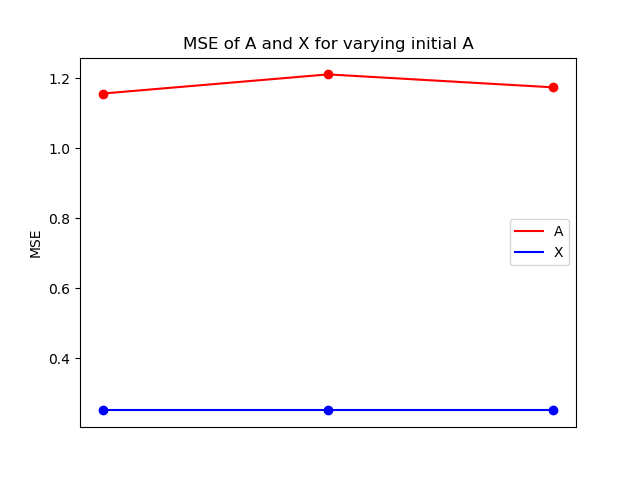
\includegraphics[scale=0.5]{figures/chapter6/Mix_Error_initial_A_m8_k16_L1000_RealA.png}
		\subcaption{Simple Data Set - Real A}
    \end{minipage} 
    \hfill
    \begin{minipage}[t]{.45\textwidth}
        \centering
		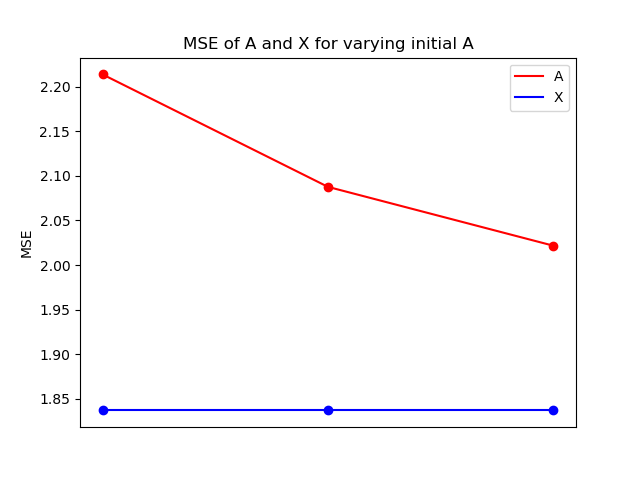
\includegraphics[scale=0.5]{figures/chapter6/AR_Error_initial_A_m8_k16_L1000_RealA.png}
		\subcaption{Autoregressive Data Set - Real A}
    \end{minipage}
\caption{}
\label{fig:initialA}
\end{figure}
\noindent
The MSE values of each tests -- estimated and real mixing matrix $\mathbf{A}$ -- can be seen in table \ref{tab:iniA}. For the real mixing matrix the MSE values of source matrix $\mathbf{X}$ are identical because the real mixing matrix is not influenced by the three different initial $\mathbf{A}_{\text{ini}}$.
\begin{table}[H]
\begin{minipage}{.5\linewidth}
\centering
\begin{tabular}{|c|c|c|c|}
\hline 
 & $\mathbf{A1}$ & $\mathbf{A2}$ & $\mathbf{A3}$ \\ 
\hline 
MSE of $\mathbf{A}$ & 1.16 & 1.21 & 1.17 \\ 
\hline 
MSE of $\mathbf{X}$ & 0.69 & 0.66 & 0.81 \\ 
\hline 
\end{tabular} 
\subcaption{Simple Data Set - estimated $\mathbf{A}$}
\end{minipage}
\begin{minipage}{.5\linewidth}
\centering
\begin{tabular}{|c|c|c|c|}
\hline
 & $\mathbf{A1}$ & $\mathbf{A2}$ & $\mathbf{A3}$ \\ 
\hline 
MSE of $\mathbf{A}$ & 2.21 & 2.09 & 2.02 \\ 
\hline 
MSE of $\mathbf{X}$ & 8.43 & 9.55 & 8.93 \\ 
\hline
\end{tabular} 
\subcaption{Autoregressive Data Set - estimated $\mathbf{A}$}
\end{minipage}
\begin{minipage}{.5\linewidth}
\centering
\begin{tabular}{|c|c|c|c|}
\hline 
 & $\mathbf{A1}$ & $\mathbf{A2}$ & $\mathbf{A3}$ \\ 
\hline 
MSE of $\mathbf{A}$ & $\times$ & $\times$ & $\times$ \\ 
\hline 
MSE of $\mathbf{X}$ & 0.25 & 0.25 & 0.25 \\ 
\hline 
\end{tabular} 
\subcaption{Simple Data Set - real $\mathbf{A}$}
\end{minipage}
\begin{minipage}{.5\linewidth}
\centering
\begin{tabular}{|c|c|c|c|}
\hline
 & $\mathbf{A1}$ & $\mathbf{A2}$ & $\mathbf{A3}$ \\ 
\hline 
MSE of $\mathbf{A}$ & $\times$ & $\times$ & $\times$ \\ 
\hline 
MSE of $\mathbf{X}$ & 1.84 & 1.84 & 1.84 \\ 
\hline
\end{tabular} 
\subcaption{Autoregressive Data Set - real $\mathbf{A}$}
\end{minipage}
\caption{(a) This are the MSE values achieve from the simple data set and (b) is the MSE values achieved from the autoregressive data set.}
\label{tab:iniA}
\end{table}
\noindent
From \ref{tab:iniA} we see that the MSE values for our estimated mixing matrix $\mathbf{A}$ are overall small compared to both data sets. However, if we look at the results for the source matrix there are a big different from the simple data set and the autoregressive data set and comparing it to the results with the real mixing matrix. 
As the autoregressive data set have a higher amplitude in the data than the simple data set, the error will become larger. 

If we look at the initial $\mathbf{A}_{\text{ini}}$ drawn from the Gaussian distribution we have a small error for the mixing matrix in the autoregressive data set while the error from the simple data set also is low. The error for source matrix is the highest value for the simple data set but comes second in the autoregressive data set. As we want to take into account that the autoregressive data set resemble the EEG measurement most we conclude that the initial $\mathbf{A}_{\text{ini}}$ from the Gaussian distribution would be the best choice in Cov-DL.
\todo[inline]{Det er en lidt lang smøre her måske, ville det gøre noget hvis man fjernede X mse her, påvirker den valgt for det burde den vel egentlig ikke i hvert fald.\\
Fortæller vi at det en gennemsnitlig fejl og over hvor meget? }

\subsubsection{Segmentation in Cov-DL}
For the Cov-DL algorithm when estimating the mixing matrix $\mathbf{A}$ the measurement matrix is transformed into the covariance domain as part of the recovering process. During the transformation the measurement matrix $\mathbf{Y}$ is divided into segments consisting of $L_s$ samples each.
During this test we will be looking how many samples $L_s$ each segment can have and how this affect the performance of the algorithms.

The system of interest to be tested on is when we have $M = 8$, $k = 16$ and $L = 1000$ samples. With $k = 16$ the number of segments can not be less than the number of active sources. For this system each segment can have maximum $L_s = 62$ corresponding to 16 segments. 
For the test, six different number of samples within each segments will be tested, $L_s = \{ 10, 20, 30, 40, 50, 60 \}$.
\begin{figure}[H]
\centering
    \begin{minipage}[t]{.45\textwidth}
        \centering
		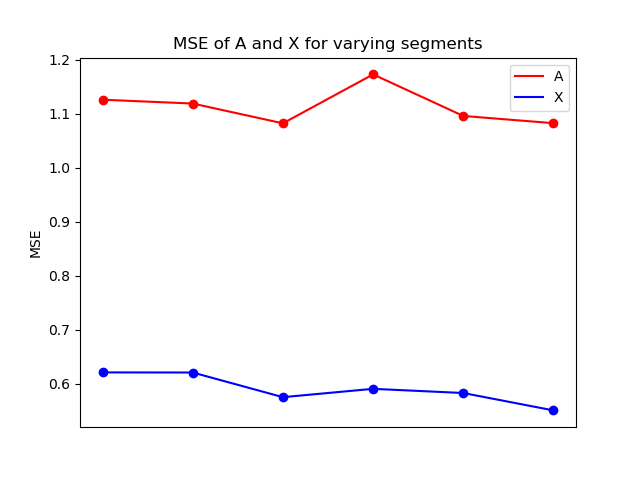
\includegraphics[scale=0.5]{figures/chapter6/Mix_Error_vary_covseg_m8_k16_L1000}
		\subcaption{Simple Data Set - Estimated A}
    \end{minipage} 
    \hfill
    \begin{minipage}[t]{.45\textwidth}
        \centering
		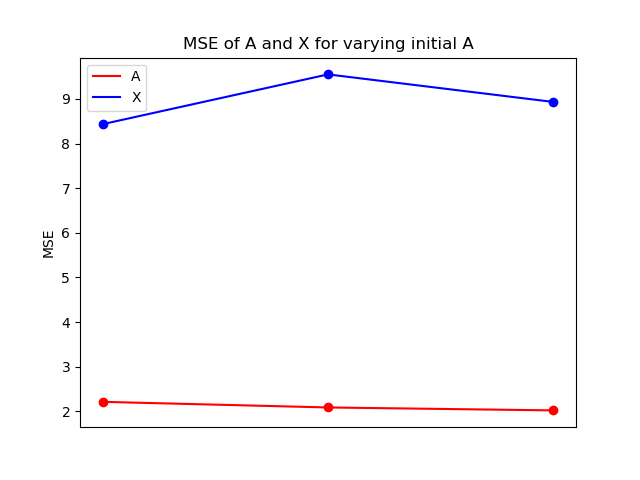
\includegraphics[scale=0.5]{figures/chapter6/AR_Error_initial_A_m8_k16_L1000.png}
		\subcaption{Autoregressive Data Set - Estimated A}
    \end{minipage}
    \begin{minipage}[t]{.45\textwidth}
        \centering
		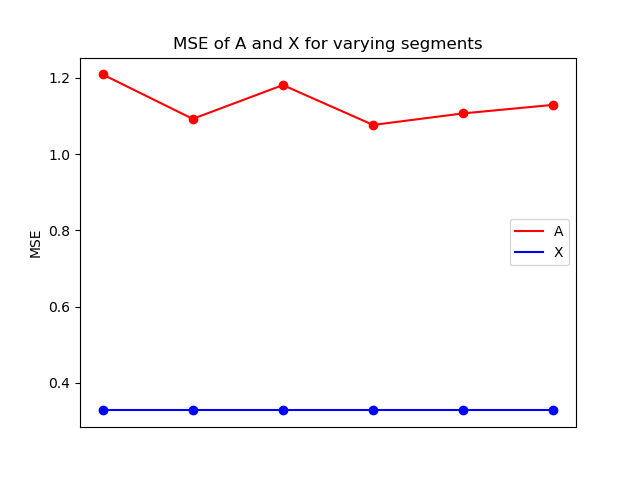
\includegraphics[scale=0.5]{figures/chapter6/Mix_Error_vary_covseg_m8_k16_L1000_RealA.png}
		\subcaption{Simple Data Set - Real A}
    \end{minipage} 
    \hfill
    \begin{minipage}[t]{.45\textwidth}
        \centering
		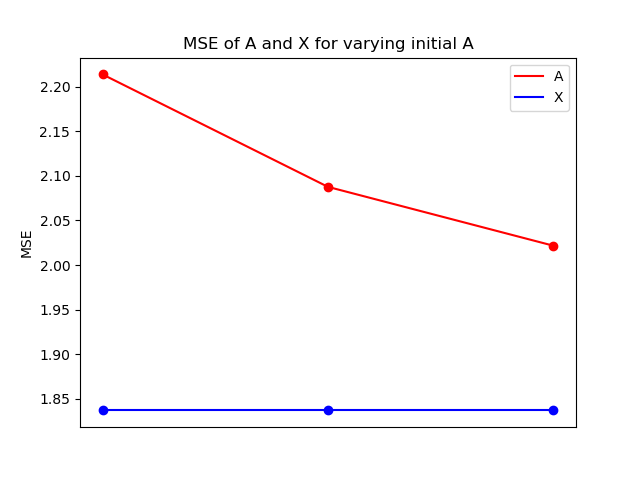
\includegraphics[scale=0.5]{figures/chapter6/AR_Error_initial_A_m8_k16_L1000_RealA.png}
		\subcaption{Autoregressive Data Set - Real A}
    \end{minipage}
\caption{}
\label{fig:seg}
\end{figure}
\noindent
The MSE values of each tests -- estimated and real mixing matrix $\mathbf{A}$ -- can be seen in table \ref{tab:seg}\todo[inline]{hvordan kan det være der kun er 3 punkter for AR dataen?\\
\textbf{X} fejlen er mærkelig høj her, er der en grund til det}.
\begin{table}[H]
\centering
\begin{minipage}{.45\textwidth}
\centering
\begin{tabular}{|c|c|c|c|c|c|c|}
\hline 
 & 10 & 20 & 30 & 40 & 50 & 60 \\ 
\hline 
MSE of $\mathbf{A}$ & 1.21 & 1.09 & 1.18 & 1.08 & 1.11 & 1.13 \\ 
\hline 
MSE of $\mathbf{X}$ & 0.69 & 0.64 & 0.68 & 0.64 & 0.65 & 0.64 \\ 
\hline 
MSE of $\mathbf{X}$ with real $\mathbf{A}$ & 0.33 & 0.33 & 0.33 & 0.33 & 0.33 & 0.33 \\ 
\hline
\end{tabular} 
\subcaption{Simple Data Set - estimated $\mathbf{A}$}
\end{minipage}
\\
\begin{minipage}{.45\textwidth}
\centering
\begin{tabular}{|c|c|c|c|c|c|c|}
\hline 
 & 10 & 20 & 30 & 40 & 50 & 60 \\ 
\hline
MSE of $\mathbf{A}$ & 1.87 & 1.90 & 1.70 & 1.92 & 1.85 & 1.88 \\
\hline 
MSE of $\mathbf{X}$ & 7.61 & 8.06 & 8.34 & 8.28 & 8.12 & 7.23 \\ 
\hline
MSE of $\mathbf{X}$ with real $\mathbf{A}$ & 2.15 & 2.15 & 2.15 & 2.15 & 2.15 & 2.15 \\  
\hline
\end{tabular} 
\subcaption{Autoregressive Data Set - estimated $\mathbf{A}$}
\end{minipage}
\caption{(a) This are the MSE values achieve from the simple data set and (b) is the MSE values achieved from the autoregressive data set.}
\label{tab:seg}
\end{table}
\noindent
Overall, in table \ref{tab:seg} there is not a big variation between the MSE values of both the simple data set and the autoregressive data set. One could argument that the number of samples within each segment does not affect the performance of the algorithms as much and therefore is more free choice. This can be seen as in the autoregressive data set the test with most and fewest samples have the smallest error.